\chapter{El Problema: Juego de Distribuci\'on de la Cerveza}

%The purpose of the game is to understand the distribution side dynamics of a multi-echelon supply chain used to distribute a single item, in this case, cases of beer.


%There is a one-point cost for holding excess inventory and a one-point cost for any backlog (old backlog + orders - current inventory).

%The game is used to illustrate one of the links between System Dynamics theory and the Feedback Control Theory which inspired it - that systems with positive feedback loops and high gain can lead to oscillation and overload,


\textit{The Beer Distribution Game}, planteado por primera vez en la Escuela de Administraci\'on y Direcci\'on de Empresas Sloan del MIT en los años 60 para ejemplificar el \textit{efecto l\'atigo}, llamado as\'i por la similaridad que tiene el comportamiento la informaci\'on en cada nivel de la cadena con el patr\'on ondulado que toma un l\'atigo, en el cual existe una mayor amplitud de onda (comparable con el ruido o la varianza en la informaci\'on) al alejarse del punto de origen (comparable al consumidor). \\

En su forma de juego de mesa, se presenta com\'unmente a alumnos reci\'en ingresados a distintas escuelas de negocios. El MIT public\'o un art\'iculo noticiero corto de \citet{Dizikes} en el cual se nota que, independientemente del rol que jueguen y de cu\'anta experiencia y preparaci\'on en negocios tengan, los humanos consistentemente fallan en encontrar la estrategia para maximizar la utilidad. Asimismo, nota que es inevitable la frustraci\'on, y que incluso los equipos que obtienen los mejores resultados del juego terminan lejos del \'optimo. \\

El \textit{Beer Distribution Game} ejemplifica la relaci\'on causal entre la toma de decisiones de cada agente con el comportamiento de todo el sistema, en este caso una cadena de suministro. Asimismo, presenta el efecto l\'atigo claramente: el retraso en la informaci\'on  causa que, a trav\'es del tiempo, el comportamiento de cada agente se vuelva menos constante cuanto m\'as lejos se encuentre del consumidor final. Por \'ultimo, evidencia las ineficiencias inherentes a tratar de resolver el problema enfoc\'andose en los agentes, ignorando que es un sistema completo. 


\section{Principales caracter\'isticas}

El juego consiste, a grandes rasgos, en asignar a cada agente un rol en una cadena de suministro de cerveza, buscando maximizar las ganancias individuales al final del juego.\\

Existen cuatro jugadores: minorista (\textit{retail}), mayorista (\textit{wholesale}), distribuidor (\textit{regional warehouse}) y f\'abrica (\textit{factory}). Dentro del juego transcurren 52 semanas (un a\~no), durante las cuales existe una demanda del consumidor, que se revela al inicio de la semana. De esta manera, el minorista debe cubrir (restringido a su inventario) la demanda del consumidor, y decidir la orden que pedir\'a al mayorista para recibir la siguiente semana. Cada jugador sigue instrucciones similares, con el objetivo de maximizar sus ganancias al final del juego.\\

Todos los agentes cuentan con un inventario inicial de cajas de cerveza,  y deben manejar correctamente su inventario para poder cumplir con la demanda del agente previo, al tiempo de minimizar los costos de almacenamiento por cada caja. Todos reciben ingresos por vender cajas de cerveza, e incurren en costos por comprar inventario, almacenar inventario, y por \'ultimo, una penalizaci\'on por no cubrir las \'ordenes.\\

La estructura del juego se puede observar en la figura \ref{diagram_wikipedia}.\footnote{Iconos creados por Freepik, Iconnice, Roundicons en \textit{www.flaticon.com}}\\


\begin{figure}[h]
\caption{Distribución de Cerveza}
\label{diagram_wikipedia}
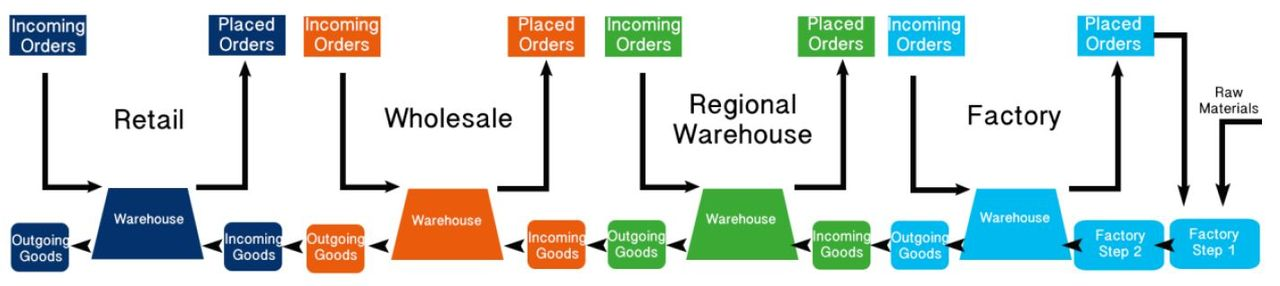
\includegraphics[width=8cm]{Diagrama_Wikipedia.JPG}
\centering
\end{figure}

De esta manera, las variables que tienen efecto en este problema son:

\begin{itemize}
    \item Demanda del consumidor
    \item Precio de la cerveza
    \item Costo de almacenaje
    \item Costo de oportunidad por \'ordenes no cumplidas
    \item Inventario inicial
\end{itemize}

Todas las variables, menos la demanda del consumidor y la producci\'on en los campos, pueden ser declaradas para el sistema (igual para todos los agentes) o individualmente (diferente para cada agente). Como se ver\'a m\'as adelante, el sistema es sumamente sensible a peque\~nos cambios en cualquiera de las variables; por ejemplo, si un agente comienza el juego con suficiente inventario para todo el a\~no, el agente superior nunca podr\'a venderle cerveza e incurrir\'a solamente en costos por almacenaje.

\subsection{Efecto Látigo}

El \textit{Efecto Látigo} se ejemplifica con el siguiente escenario:


\begin{enumerate}
    \item El comprador, que generalmente compra $6$ cervezas, ahora quiere $10$, pero la tienda minorista solamente cuenta con $7$. El minorista le venderá todo su inventario, pues es la acci\'on que maximiza su ganancia. Debe decidir si volverá a tener un inventario de $6$ o si debe pedir un número mayor de cervezas, atendiendo la aparentemente creciente demanda. Decide pedir $9$ cervezas al siguiente nivel, la tienda de mayoreo.
    \item El mayorista cuenta con $17$ cervezas. Llena el pedido del minorista, pero decide que ten\'ia guardado demasiado inventario, as\'i que se queda con $8$ cervezas en su almac\'en, sin hacer una orden al siguiente nivel, la tienda de distribución.
    \item La tienda de distribuci\'on decide no comprar unidades a la f\'abrica, dado que no disminuy\'o su inventario.
    \item La f\'abrica conoce la restricci\'on de estacionalidad de la cebada, as\'i que compra una m\'inima cantidad a los campos.
\end{enumerate}

En este escenario, el mayorista obtuvo informaci\'on distorsionada acerca del repentino crecimiento en la demanda del comprador, mientras que la tienda de distribución podr\'ia incluso interpretar que el comprador disminuy\'o su consumo. Si este comportamiento se mantiene durante algunos periodos más, recibiría la noticia (por medio de un incremento en las órdenes regulares) con un retraso considerable.\\

El \textit{Efecto L\'atigo} s\citet{Strozzi}e refiere precisamente a este fenómeno: mientras m\'as ``arriba'' en la cadena de suministro se encuentre un agente (es decir, m\'as lejos del contacto directo con el comprador), m\'as distorsionada es la informaci\'on que tiene acerca de la verdadera demanda del comprador.

\section{Acercamiento en el Presente Trabajo}

Este problema se ha estudiado antes por \citet{Strozzi}, por medio de Algoritmos Genéticos y por \citet{Chaharsooghi} por medio de $Q-learning$. Ambas metodolog\'ias ser\'an abordadas en el siguiente cap\'itulo.\\

El aporte de este trabajo será agregar un componente de estacionalidad en el proveedor de la f\'abrica: el campo.